\documentclass{beamer}
%
% Choose how your presentation looks.
%
% For more themes, color themes and font themes, see:
% http://deic.uab.es/~iblanes/beamer_gallery/index_by_theme.html
%
\mode<presentation>
{
  \usetheme{AnnArbor}      % or try Darmstadt, Madrid, Warsaw, ...
  \usecolortheme{default} % or try albatross, beaver, crane, ...
  \usefonttheme{default}  % or try serif, structurebold, ...
  \setbeamertemplate{navigation symbols}{}
  \setbeamertemplate{caption}[numbered]
} 

\usepackage[english]{babel}
\usepackage[utf8x]{inputenc}
\usepackage{hyperref}
\hypersetup{colorlinks=true}
\usepackage{graphicx}
\graphicspath{{./figures/}}
\usepackage{caption}
\usepackage{subcaption}
\usepackage{amsmath}
\usepackage{biblatex}
\addbibresource{bibliography.bib}

% From https://tex.stackexchange.com/a/178803/273247
\AtBeginSection[]{
  \begin{frame}
  \vfill
  \centering
  \begin{beamercolorbox}[sep=8pt,center,shadow=true,rounded=true]{title}
    \usebeamerfont{title}\insertsectionhead\par%
  \end{beamercolorbox}
  \vfill
  \end{frame}
}

\title[NNs, GPs, and Their Siblings]{
Neural Networks, Gaussian Processes, and \\
Their Siblings
}
%\author{Victor Verma}
\author[Victor Verma]{Victor Verma}
\institute[]{Hot Ideas in Machine Learning Reading Group, University of Michigan}
\date{7/15/22}

\begin{document}

\begin{frame}
  \titlepage
\end{frame}

% Uncomment these lines for an automatically generated outline.
\begin{frame}{Outline}
    \tableofcontents
\end{frame}

\section{Neural Networks}

\begin{frame}{Introduction}
    A \textbf{neural network (NN)} is a differentiable function that can be represented by a graph in which nodes represent primitive operations like matrix multiplication and edges or connections represent numeric data like vectors and matrices. See Fig.~\ref{fig:mlp} for an example.
    
    \medskip
    
    Nodes are called \textbf{neurons}; edges are called \textbf{connections}. Connections have \textbf{weights} that are used to scale inputs. Let $\boldsymbol{x}$ be the vector of inputs for a neuron; let $\boldsymbol{w}$ be the vector of corresponding weights; let $y$ be the output. Then
    \[
    y = \varphi(\boldsymbol{w}^T \boldsymbol{x} + b),
    \]
    where $\varphi$ is a nonlinear function called the \textbf{activation function} and $b$ is a scalar called the \textbf{bias}.
    
    \medskip
    
    Nodes are often grouped into \textbf{layers}; a NN with many layers is called \textbf{deep}.
\end{frame}

\begin{frame}{Introduction}
    \begin{figure}
        \centering
        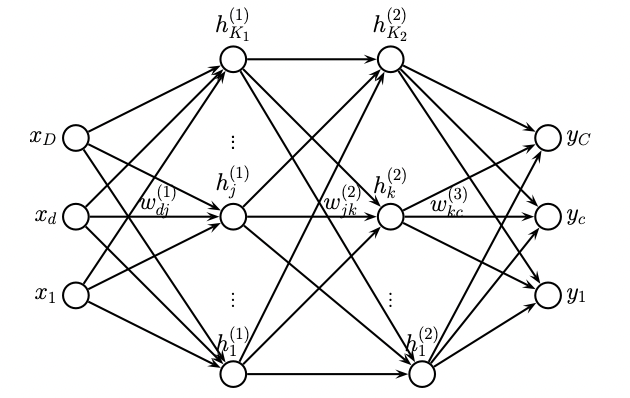
\includegraphics[scale=0.8]{mlp.png}
        \caption{A particular kind of neural network called a multi-layer perceptron \cite{pml2Book}.}
        \label{fig:mlp}
    \end{figure}    
\end{frame}

\begin{frame}{Activation Functions}
    \begin{columns}
        \column{0.55\textwidth}
            Some examples of activation functions are the \textbf{sigmoid function} $a \mapsto \frac{1}{1 + e^{-a}}$, the \textbf{rectified linear unit (ReLU)} $a \mapsto \max(a, 0)$, and the \textbf{leaky ReLU} $a \mapsto\max(a, 0) + \alpha\min(a, 0)$.
        \column{0.45\textwidth}
            \begin{figure}
                \centering
                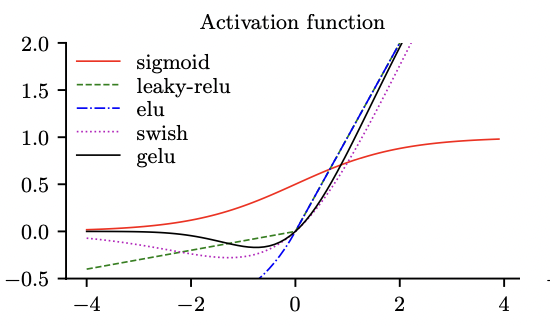
\includegraphics[scale=0.5]{activation_functions}
                \caption{Some examples of activation functions \cite{pml2Book}.}
                \label{fig:activation_functions}
            \end{figure}
    \end{columns}
\end{frame}

\begin{frame}{Multi-Layer Perceptrons (MLPs)}
    A \textbf{multi-layer perceptron (MLP)} consists of a series of \textbf{linear or fully-connected layers}. Fig.~\ref{fig:mlp} shows an example.
    
    \medskip
    
    A MLP with an input layer, one hidden layer, and an output layer can be written as
    \[
    f(\boldsymbol{x}; \boldsymbol{\theta}) = \varphi_2(\boldsymbol{W_2}\varphi_1(\boldsymbol{W_1}\boldsymbol{x} + \boldsymbol{b_1}) + \boldsymbol{b_2}).
    \]
    $\boldsymbol{W_1}$ contains the weights of the input layer-hidden layer connections, $\boldsymbol{b_1}$ contains the hidden layer neurons' biases, and $\varphi_1$ is the activation function used in the hidden layer. $\boldsymbol{W_2}$, $\boldsymbol{b_2}$, and $\varphi_2$ are defined similarly.
    
    \medskip
    
    Similar expressions can be written when there are multiple hidden layers.
\end{frame}

\begin{frame}{Convolutional Layers}
    An image can be represented as a stack of matrices associated with different \textbf{channels}. For example, there can be channels for red, blue, and green.
    
    \medskip
    
    A \textbf{filter} or \textbf{kernel} is a stack of small matrices used to extract a particular feature of an image. \textbf{Convolution} is the process of using a filter for feature extraction. Let $\boldsymbol{X} \in \mathbb{R}^{H \times W \times C}$ be a $C$-channel $H \times W$ image. Let $W^{(d)} \in \mathbb{R}^{h \times w \times C}$ be the $d$th filter for $d = 1, \ldots, D$. Convolution produces a $D$-channel image; the $(i, j)$-entry in channel $d$ is
    \[
    \sum_{c = 0}^{C - 1} \sum_{u = 0}^{h - 1} \sum_{v = 0}^{w - 1} x_{i + u, j + v, c}w_{u, v, c}^{(d)}.
    \]
    See Fig.~\ref{fig:convolutional_layer} for an example.
\end{frame}

\begin{frame}{Convolutional Layers}
    \begin{figure}
        \centering
        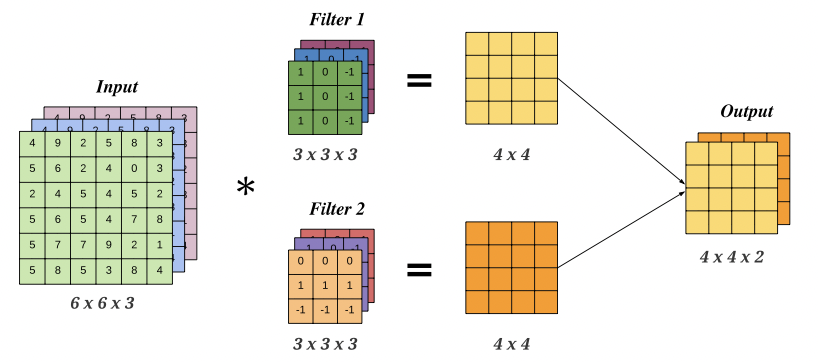
\includegraphics[scale=0.8]{convolutional_layer}
        \caption{A convolutional layer with three input and two output channels \cite{pml2Book}.}
        \label{fig:convolutional_layer}
    \end{figure}
\end{frame}

\begin{frame}{Convolutional Neural Networks (CNNs)}
    A \textbf{pooling layer} performs dimensionality reduction by taking the maximum or average over a patch.

    \medskip

    A convolutional neural network (CNN) consists of a series of convolutional layers, pooling layers, and linear layers. CNNs are frequently used in computer vision. Fig.~\ref{fig:cnn} shows a CNN used to classify images of handwritten digits.
\end{frame}

\begin{frame}{Convolutional Neural Networks (CNNs)}
    \begin{figure}
        \centering
        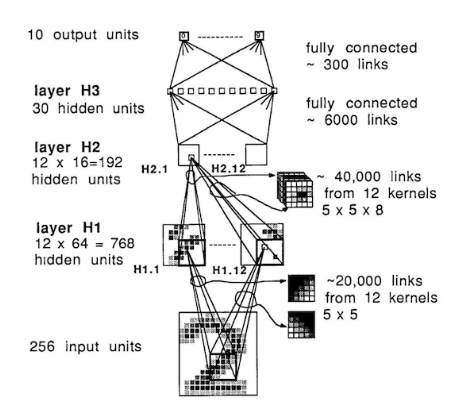
\includegraphics[scale=0.8]{cnn}
        \caption{A CNN used to classify images of handwritten digits \cite{pml2Book}.}
        \label{fig:cnn}
    \end{figure}
\end{frame}

\section{Bayesian Neural Networks}

\begin{frame}{Bayesian Neural Networks}
    Bayesian Neural Networks
\end{frame}

\begin{frame}{Introduction}
    For a deep neural network, there can be many parameter settings for which the fit to the training data is good. Different settings can give rise to very different fitted models. It turns out that we can achieve good generalization by combining these models instead of using just one. \textbf{Bayesian neural networks (BNNs)} provide a means for doing this.
    
    \medskip
    
    We start with a prior $p(\boldsymbol{\theta})$ over the parameters. We then compute the posterior $p(\boldsymbol{\theta} | \mathcal{D})$ and use Bayesian model averaging to compute the posterior predictive density
    \begin{equation*}
        p(\boldsymbol{y} | \boldsymbol{x}, \mathcal{D}) = \int p(\boldsymbol{y} | \boldsymbol{x}, \boldsymbol{\theta})p(\boldsymbol{\theta} | \mathcal{D})\,d\boldsymbol{\theta}.
    \end{equation*}
\end{frame}

\begin{frame}{Gaussian priors}
    Let
    \[
    f(\boldsymbol{x}; \boldsymbol{\theta}) = \boldsymbol{W_L}(\cdots\varphi(\boldsymbol{W_1}\boldsymbol{x} + \boldsymbol{b_1})) + \boldsymbol{b_L};
    \]
    this is a multi-layer perceptron (MLP) with $L - 1$ layers and activation function $\varphi$. When $L = 1$, this becomes
    \[
    f(\boldsymbol{x}; \boldsymbol{\theta}) = \boldsymbol{W_2}\varphi(\boldsymbol{W_1}\boldsymbol{x} + \boldsymbol{b_1}) + \boldsymbol{b_2}.
    \]
    Specifying a prior entails specifying the distributions of the $\boldsymbol{W}_{\ell}$'s and the $\boldsymbol{b}_{\ell}$'s. Typically, Gaussian priors are used: $\boldsymbol{W}_{\ell} \sim \mathcal{N}(\boldsymbol{0}, \alpha_{\ell}^2\boldsymbol{I})$ and $\boldsymbol{b}_{\ell} \sim \mathcal{N}(\boldsymbol{0}, \beta_{\ell}^2\boldsymbol{I})$ for $\ell = 1, \ldots, L$.
\end{frame}

\begin{frame}{Gaussian priors}
    Let $L = 2$, let $\varphi$ be the sigmoid function, and let the input and output be linear. Each panel of Fig.~\ref{fig:mlp_priors} shows a sample of MLPs from a particular Gaussian prior.
    \begin{figure}
        \centering
        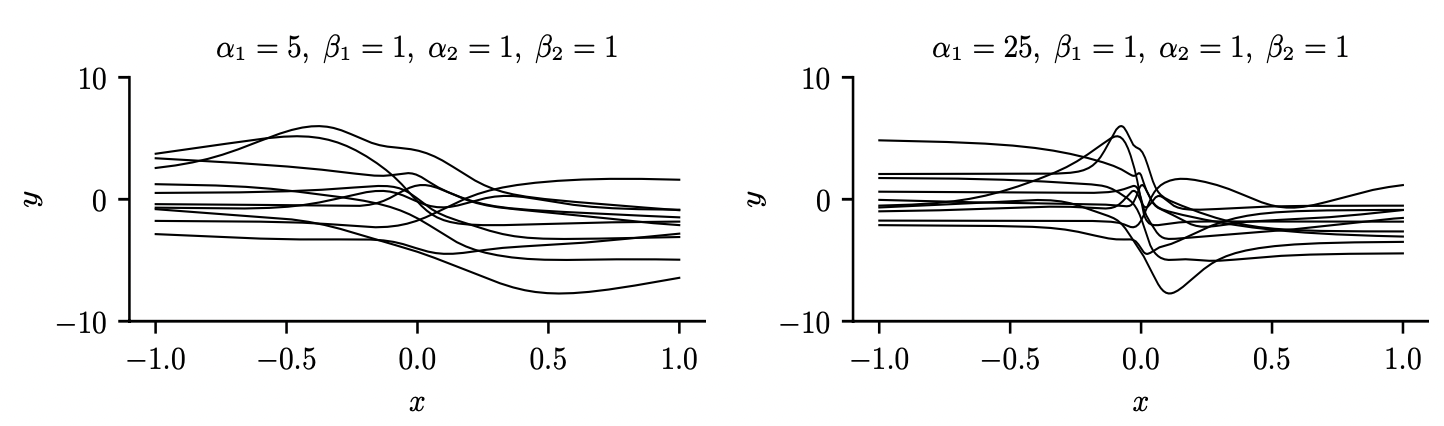
\includegraphics[width=\textwidth]{mlp_priors}
        \caption{Samples of MLPs from two different Gaussian priors \cite{pml2Book}.}
        \label{fig:mlp_priors}
    \end{figure}
\end{frame}

\begin{frame}{Learning the prior}
    In more general situations, there are a few approaches that can be taken to choosing a prior:
    \begin{itemize}
        \item Cross-validation can be used to identify a good choice of hyperparameters, but it can be slow if there are many hyperparameters.
        \item An empirical Bayes approach can be taken. E.g., if the hyperparameters are $\boldsymbol{\alpha}$ and $\boldsymbol{\beta}$, we could find the values that maximize $\log p(\mathcal{D} | \boldsymbol{\alpha}, \boldsymbol{\beta}) = \int \log p(\mathcal{D} | \boldsymbol{\theta})p(\boldsymbol{\theta} | \boldsymbol{\alpha}, \boldsymbol{\beta})\,d\boldsymbol{\theta}$. However, this can be computationally difficult.
        \item A third approach is Bayesian transfer learning: estimating the posterior using one dataset and then using it as the prior with another dataset.
    \end{itemize}
\end{frame}

\begin{frame}{Likelihoods for BNNs}
    There are two ways to transform the likelihood $p(\boldsymbol{y} | \boldsymbol{x}, \boldsymbol{\theta})$ to get better predictive accuracy. Ordinarily we would have $p(\boldsymbol{\theta} | \mathcal{D}) \propto p(\boldsymbol{y} | \boldsymbol{x}, \boldsymbol{\theta})p(\boldsymbol{\theta})$, or $\log p(\boldsymbol{\theta} | \mathcal{D}) = \log p(\boldsymbol{y} | \boldsymbol{x}, \boldsymbol{\theta}) + \log p(\boldsymbol{\theta}) + \text{const}$.
    \begin{itemize}
        \item One approach is to use a \textbf{tempered posterior}: $\log p_{\text{tempered}}(\boldsymbol{\theta} | \mathcal{D}) = \alpha\log p(\boldsymbol{y} | \boldsymbol{x}, \boldsymbol{\theta}) + \log p(\boldsymbol{\theta}) + \text{const}$.
        \item Another approach is to use a \textbf{cold posterior}: $\log p_{\text{cold}}(\boldsymbol{\theta} | \mathcal{D}) = \frac{1}{T}\log p(\boldsymbol{y} | \boldsymbol{x}, \boldsymbol{\theta}) + \frac{1}{T}\log p(\boldsymbol{\theta}) + \text{const}$.
    \end{itemize}
    Model selection methods like cross-validation can be used to choose $\alpha$ and $T$.
\end{frame}

\begin{frame}{Posteriors for BNNs}
    There are several ways to approximate the posterior:
    \begin{itemize}
        \item Laplace approximation
        \item Variational inference
        \item Expectation propagation
        \item Last layer methods
        \item Dropout
        \item MCMC methods
        \item Methods based on the SGD trajectory
        \item Deep ensembles
    \end{itemize}
\end{frame}

\begin{frame}{Laplace approximation}
    Let $\mathcal{E}(\boldsymbol{\theta}) = -\log p(\boldsymbol{\theta}, \mathcal{D})$; $\mathcal{E}$ is called the \textbf{energy}. Then $p(\boldsymbol{\theta} | \mathcal{D}) \propto e^{-\mathcal{E}(\boldsymbol{\theta})}$.
    Letting $\hat{\boldsymbol{\theta}}$ be the MAP estimate, we have
    \begin{align*}
        \mathcal{E}(\boldsymbol{\theta}) &\approx \mathcal{E}(\hat{\boldsymbol{\theta}}) + (\boldsymbol{\theta} - \hat{\boldsymbol{\theta}})^T \nabla\mathcal{E}(\hat{\boldsymbol{\theta}}) + \frac{1}{2}(\boldsymbol{\theta} - \hat{\boldsymbol{\theta}})^T \boldsymbol{H}(\boldsymbol{\theta} - \hat{\boldsymbol{\theta}}) \\
        &\approx \mathcal{E}(\hat{\boldsymbol{\theta}}) + \frac{1}{2}(\boldsymbol{\theta} - \hat{\boldsymbol{\theta}})^T \boldsymbol{H}(\boldsymbol{\theta} - \hat{\boldsymbol{\theta}}) \\
        p(\boldsymbol{\theta}, \mathcal{D}) &\approx e^{-\mathcal{E}(\hat{\boldsymbol{\theta}})}\exp\left[-\frac{1}{2}(\boldsymbol{\theta} - \hat{\boldsymbol{\theta}})^T \boldsymbol{H}(\boldsymbol{\theta} - \hat{\boldsymbol{\theta}})\right] \\
        p(\boldsymbol{\theta} | \mathcal{D}) &\approx \text{constant} \cdot \exp\left[-\frac{1}{2}(\boldsymbol{\theta} - \hat{\boldsymbol{\theta}})^T \boldsymbol{H}(\boldsymbol{\theta} - \hat{\boldsymbol{\theta}})\right].
    \end{align*}
    Hence, $p(\boldsymbol{\theta} | \mathcal{D}) \approx \mathcal{N}(\boldsymbol{\theta} | \hat{\boldsymbol{\theta}}, \boldsymbol{H}^{-1})$, the \textbf{Laplace approximation} to $p(\boldsymbol{\theta} | \mathcal{D})$.
\end{frame}

\begin{frame}{Laplace approximation}
    Let $\boldsymbol{f}(\boldsymbol{x}; \boldsymbol{\theta}) \in \mathbb{R}^C$ be a neural network, where $\boldsymbol{\theta} \in \mathbb{R}^P$. Let $\boldsymbol{J}_{\boldsymbol{\theta}}(\boldsymbol{x}) \in \mathbb{R}^{C \times P}$ be the Jacobian of $\boldsymbol{f}$. Let $\boldsymbol{\Lambda}(\boldsymbol{y}; \boldsymbol{f}) = -\nabla_{\boldsymbol{f}}^2\log p(\boldsymbol{y} | \boldsymbol{f})$; this is the per-input noise term.
    
    \medskip

    If we use a Gaussian prior, $p(\boldsymbol{\theta}) = \mathcal{N}(\boldsymbol{\theta} | \boldsymbol{m}_0, \boldsymbol{S}_0)$, then the Laplace approximation to the posterior $p(\boldsymbol{\theta} | \mathcal{D})$ will be the $\mathcal{N}(\hat{\boldsymbol{\theta}}, \boldsymbol{\Sigma}_{\text{GGN}})$ distribution, where $\hat{\boldsymbol{\theta}}$ is the MAP estimate and
    \[
    \boldsymbol{\Sigma}_{\text{GGN}} = \left(\sum_{n = 1}^N \boldsymbol{J}_{\hat{\boldsymbol{\theta}}}(\boldsymbol{x}_n)^T\boldsymbol{\Lambda}(\boldsymbol{y}_n; \boldsymbol{f}_n)\boldsymbol{J}_{\hat{\boldsymbol{\theta}}}(\boldsymbol{x}_n) + \boldsymbol{S}_0^{-1}\right)^{-1}.
    \]
\end{frame}

\begin{frame}{Methods based on the SGD trajectory}
    Under certain assumptions, with a fixed learning rate, iterates produced by stochastic gradient descent can be viewed as samples from a Gaussian approximation $\mathcal{N}(\boldsymbol{\theta} | \hat{\boldsymbol{\theta}}, \boldsymbol{\Sigma})$ to $p(\boldsymbol{\theta} | \mathcal{D})$, where $\hat{\boldsymbol{\theta}}$ is a local mode. With a constant learning rate, the sequence of iterates $\{\boldsymbol{\theta}_s\}$ doesn't converge to a local optimum. However, they do lie along the periphery of a point of good generalization. \textbf{Stochastic Weight Averaging (SWA)} computes $\bar{\boldsymbol{\theta}} = \sum_{s = 1}^S \boldsymbol{\theta}_s$, which should produce better generalization.
    
    \begin{figure}
        \centering
        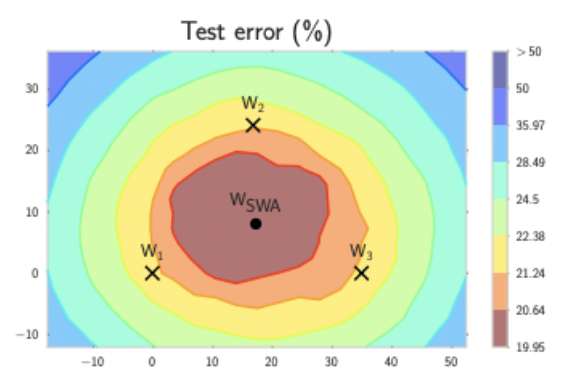
\includegraphics[scale=0.5]{stochastic_weight_averaging}
        \caption{An example instance of SWA \cite{pml2Book}.}
        \label{fig:stochastic_weight_averaging}
    \end{figure}
\end{frame}

\begin{frame}{Methods based on the SGD trajectory}
    \textbf{Stochastic Weight Averaging with Gaussian Posterior (SWAG)} is an extension of SWA that approximates the posterior using a Gaussian distribution centered at the SWA solution. The approximation is $\mathcal{N}(\boldsymbol{\theta} | \hat{\boldsymbol{\theta}}, \boldsymbol{\Sigma})$, where $\hat{\boldsymbol{\theta}}$ is as on the previous slide and $\boldsymbol{\Sigma}$ is the sum of a diagonal matrix and a low-rank matrix computed from $\boldsymbol{\theta}_1, \ldots, \boldsymbol{\theta}_S$. SWAG can be used on large networks and offers improved accuracy.
\end{frame}

\begin{frame}{Deep ensembles}
    Some methods approximate $p(\boldsymbol{\theta} | \mathcal{D})$ in a neighborhood of one of its modes. However, the posterior for a deep neural network could have many modes. Fitted functions at the same mode may be quite similar, while fitted functions at different modes may be very different. So, focusing on one mode can result in underestimation of uncertainty and poor generalization.
    
    \medskip
    
    The method of \textbf{deep ensembles} instead uses multiple modes $\hat{\boldsymbol{\theta}}_1, \ldots, \hat{\boldsymbol{\theta}}_M$:
    \[
    p(\boldsymbol{\theta} | \mathcal{D}) \approx \frac{1}{M}\sum_{m = 1}^M \delta(\boldsymbol{\theta} - \hat{\boldsymbol{\theta}}_m).
    \]
    The multiple modes can be obtained by varying random seeds, hyperparameters, or architecture.
\end{frame}

\begin{frame}{Deep ensembles}
    Below are some extensions of deep ensembles:
    \begin{itemize}
        \item \textbf{Multi-SWAG} uses Gaussian distributions instead of point masses:
        \[
        p(\boldsymbol{\theta} | \mathcal{D}) \approx \frac{1}{M}\sum_{m = 1}^M \mathcal{N}(\boldsymbol{\theta} | \hat{\boldsymbol{\theta}}_m, \boldsymbol{\Sigma}_m).
        \]
        This makes it possible to generate arbitrarily many posterior samples.
        \item \textbf{Bootstrap sampling} trains different ensemble members on different subsets of the data to increase diversity in the predictions.
    \end{itemize}
\end{frame}

\begin{frame}{Approximating the posterior predictive distribution}
    Using one of the methods described on the preceding slides, we can compute an estimate $q(\boldsymbol{\theta})$ of $p(\boldsymbol{\theta} | \mathcal{D})$. Then
    \begin{align*}
        p(\boldsymbol{y} | \boldsymbol{x}, \mathcal{D}) &\approx \int q(\boldsymbol{\theta})p(\boldsymbol{y} | \boldsymbol{x}, \boldsymbol{\theta})\,d\boldsymbol{\theta} \\
        &\approx \frac{1}{S}\sum_{s = 1}^S p(\boldsymbol{y} | \boldsymbol{f}(\boldsymbol{x}, \boldsymbol{\theta}^s)),
    \end{align*}
    where $\boldsymbol{\theta}^s \sim q(\boldsymbol{\theta})$.
\end{frame}

\begin{frame}{Generalization in Bayesian deep learning}
    "Being Bayesian" can improve
    \begin{itemize}
        \item Predictive accuracy
        \item Generalization performance
    \end{itemize}
\end{frame}

\begin{frame}{Sharp vs flat minima}
    A minimum of a loss function can be \textbf{sharp} or \textbf{flat}.
    \begin{itemize}
        \item At a sharp minimum, the function has a narrow, deep hole (Fig.~\ref{fig:sharp_minimum}).
        \item At a flat minimum, it has a broad, shallow hole (Fig.~\ref{fig:flat_minimum}).
    \end{itemize}
    
    \begin{figure}
        \centering
        \begin{subfigure}[b]{0.4\textwidth}
            \centering
            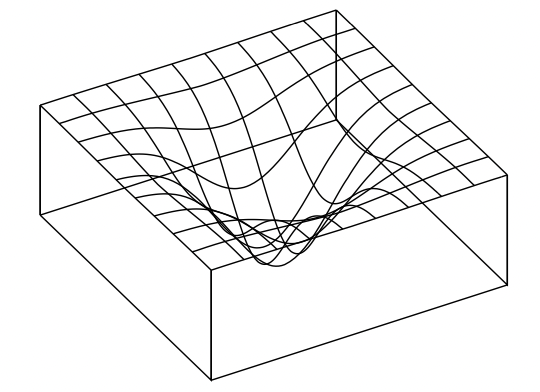
\includegraphics[width=\textwidth]{sharp_minimum}
            \caption{A sharp minimum}
            \label{fig:sharp_minimum}
        \end{subfigure}
        \begin{subfigure}[b]{0.4\textwidth}
            \centering
            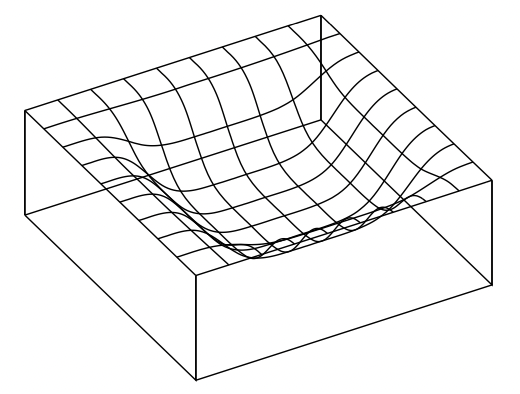
\includegraphics[width=\textwidth]{flat_minimum}
            \caption{A flat minimum}
            \label{fig:flat_minimum}
        \end{subfigure}
        \caption{Sharp and flat minima \cite{pml2Book}.}
        \label{fig:sharp_and_flat_minima}
    \end{figure}
\end{frame}

\begin{frame}{Sharp vs flat minima}
    Flat minima are preferable to sharp minima for two reasons:
    \begin{itemize}
        \item A sharp minimum corresponds to a tiny loss, which is typically caused by overfitting.
        \item Flat minima are more robust and generalize better. This can seen in two ways:
            \begin{itemize}
                \item A flat minimum corresponds to a region in parameter space with high posterior uncertainty; samples from the region don't memorize irrelevant details of the training set.
                \item A flat minimum has a short description length, i.e., few bits are needed to specify its location. This results in better generalization.
            \end{itemize}
    \end{itemize}
\end{frame}

\begin{frame}{Sharp vs flat minima}
    SGD (Stochastic Gradient Descent) tends to avoid sharp minima:
    \begin{itemize}
        \item A sharp minimum is in a region $\mathcal{A}$ of low evidence.
        \item The evidence for $\mathcal{A}$ is proportional to $\int_{\mathcal{A}} e^{-\mathcal{L}(\boldsymbol{\theta})}\,d\boldsymbol{\theta}$, so this integral is small.
        \item The integral is proportional to SGD's probability of entering $\mathcal{A}$, so SGD is unlikely to enter $\mathcal{A}$.
    \end{itemize}
    This property is due to SGD's use of noise.
\end{frame}

\begin{frame}{Effective dimensionality of a model}
    The \textbf{effective dimensionality} of a model reflects how many well-determined parameters it has. It is defined as
    \begin{equation*}
        N_{\text{eff}}(\boldsymbol{H}, c) = \sum_{i = 1}^k \frac{\lambda_i}{\lambda_i + c},
    \end{equation*}
    where $\boldsymbol{H}$ is the Hessian of the loss at the appropriate local mode, $\lambda_1, \ldots, \lambda_k$ are $\boldsymbol{H}$'s eigenvalues, and $c$ is a regularization constant.
    
    \medskip
    
    A low effective dimensionality implies that significant compression is possible. Also, the effective dimensionality is a good proxy for generalization.
\end{frame}

\begin{frame}{Effective dimensionality of a model}
    Fig.~\ref{fig:effective_dimensionality_and_test_loss} illustrates the last point on the previous slide. For CNNs with near-zero training loss, the pattern in the test loss closely resembles that in the effective dimensionality.
    \begin{figure}
        \centering
        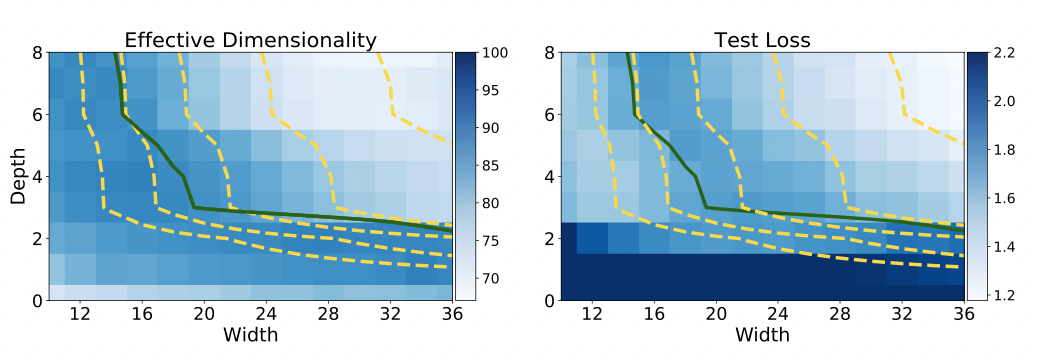
\includegraphics[width=\textwidth]{effective_dimensionality_and_test_loss}
        \caption{Effective dimensionality and test loss for various CNNs trained on the CIFAR-100 image dataset \cite{pml2Book}. CNNs above the green curve have near-zero training loss. CNNs on the same yellow curve have the same number of parameters.}
        \label{fig:effective_dimensionality_and_test_loss}
    \end{figure}    
\end{frame}

\begin{frame}{Double descent}
    For an \textbf{over-parameterized model}, there are many more parameters than training points. Surprisingly, instead of overfitting, these models often generalize well. As the number of parameters increases, we see \textbf{double descent}. The test error decreases, then increases, then decreases again, as shown in Fig.~\ref{fig:double_descent}.
    
    \begin{figure}
        \centering
        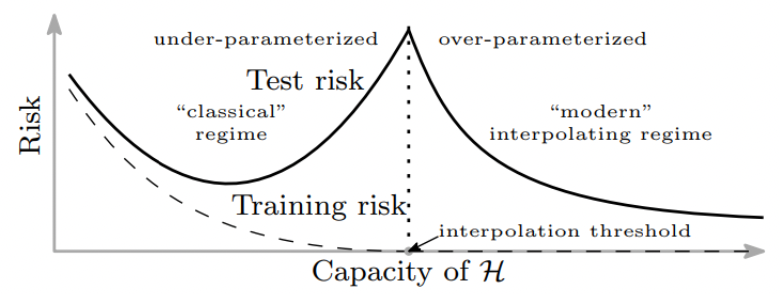
\includegraphics[width=\textwidth]{double_descent}
        \caption{Risk curves illustrating double descent \cite{pml2Book}.}
        \label{fig:double_descent}
    \end{figure}
\end{frame}

\begin{frame}{Double descent}
    Double descent can be alleviated by Bayesian model averaging. Fig.~\ref{fig:double_descent_and_bma} shows the test error of neural networks of various widths that were trained on CIFAR-100. SWAG mitigates double descent, while Multi-SWAG eliminates it.
    \begin{figure}
        \centering
        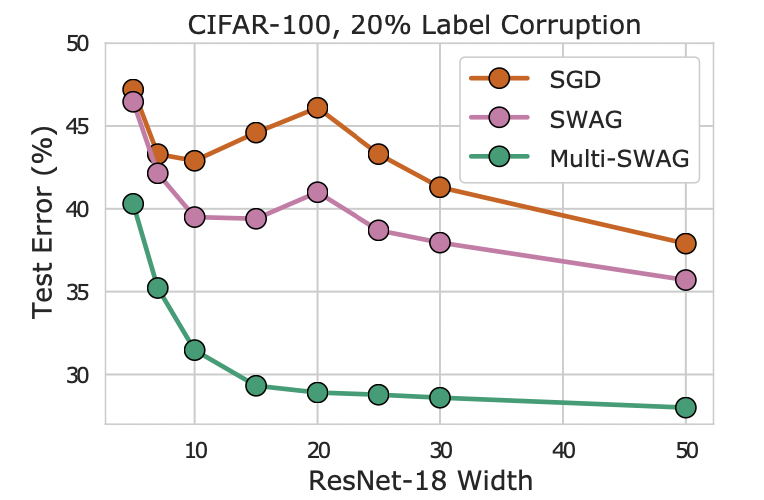
\includegraphics[scale=0.5]{double_descent_and_bma}
        \caption{An illustration of the effect of Bayesian model averaging on double descent \cite{pml2Book}.}
        \label{fig:double_descent_and_bma}
    \end{figure}
\end{frame}

\begin{frame}{Double descent}
    The effective dimensionality helps explain why double descent occurs. In Fig.~\ref{fig:double_descent_and_effective_dimensionality}, as the layer width increases, the effective dimensionality decreases, increases, and then decreases again. The lower the effective dimensionality, the better the model generalizes. This explains why the test error decreases, increases, and then decreases again.
    \begin{figure}
        \centering
        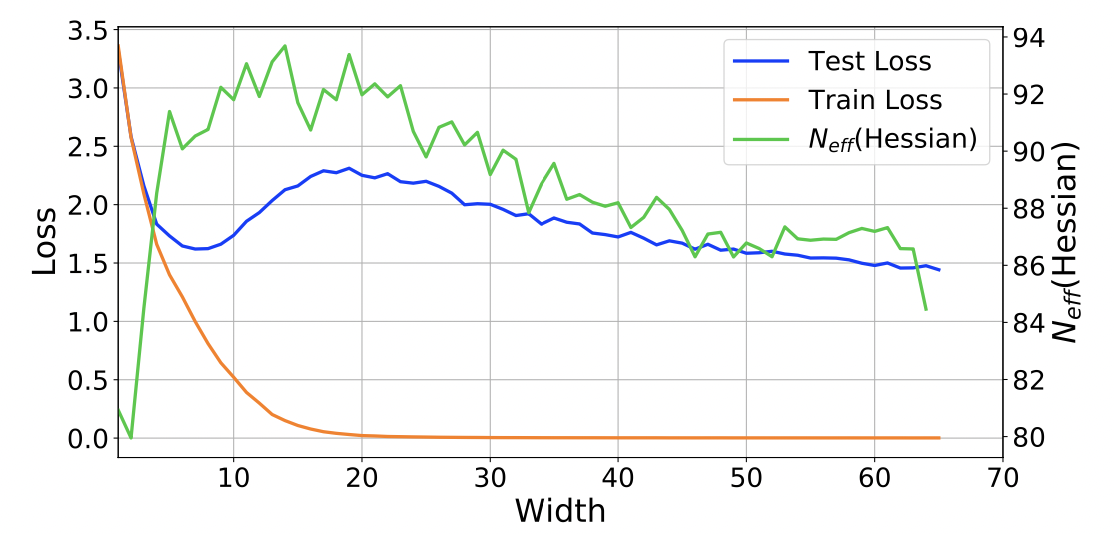
\includegraphics[scale=0.4]{double_descent_and_effective_dimensionality}
        \caption{The connection between double descent and the effective dimensionality \cite{pml2Book}.}
        \label{fig:double_descent_and_effective_dimensionality}
    \end{figure}
\end{frame}

\section{Gaussian Processes}

\begin{frame}{Introduction}
    Suppose that we have an input $\boldsymbol{x}$ and an  output $y$ related by an unknown input-output mapping $f$. We could perform inference on $f$ by putting a prior $p(f)$ on it, collecting data $\mathcal{D}$, and then computing the posterior $p(f | \mathcal{D})$.
    
    \medskip
    
    Gaussian processes provide one means for implementing this strategy. Let $f : \mathcal{X} \to \mathbb{R}$. Let $\boldsymbol{X} = \{\boldsymbol{x}_n \in \mathcal{X}\}_{n = 1}^N$ and let $\boldsymbol{f}_X = (f(\boldsymbol{x}_1), \ldots, f(\boldsymbol{x}_N))$. $f$ is a \textbf{Gaussian process (GP)} if $\boldsymbol{f}_X$ is jointly Gaussian for any $N$ and $\boldsymbol{x}_1, \ldots, \boldsymbol{x}_N$.
    
    \medskip
    
    A GP has a mean function $m(\boldsymbol{x}) \in \mathbb{R}$ and a covariance function $\mathcal{K}(\boldsymbol{x}, \boldsymbol{x}') \ge 0$. $\mathcal{K}$ is a \textbf{Mercer kernel}, which will be described shortly. We write $f(\boldsymbol{x}) \sim GP(m(\boldsymbol{x}), \mathcal{K}(\boldsymbol{x}, \boldsymbol{x}'))$.
\end{frame}

\begin{frame}{Introduction}
    The mean and covariance functions satisfy
    \begin{align*}
        m(\boldsymbol{x}) &= \mathbb{E}[f(\boldsymbol{x})] \\
        \mathcal{K}(\boldsymbol{x}, \boldsymbol{x}') &= \mathbb{E}[(f(\boldsymbol{x}) - m(\boldsymbol{x}))(f(\boldsymbol{x}') - m(\boldsymbol{x}'))^T].
    \end{align*}
    Let $\boldsymbol{X} = \{\boldsymbol{x}_1, \ldots, \boldsymbol{x}_N\}$. Let $\boldsymbol{\mu}_X = (m(\boldsymbol{x}_1), \ldots, m(\boldsymbol{x}_N))$ and let $\boldsymbol{K}_{X, X}$ be the $N \times N$ matrix whose $(i, j)$-entry is $\mathcal{K}(\boldsymbol{x}_i, \boldsymbol{x}_j)$. Since $\boldsymbol{f}_X$ is multivariate Gaussian, $p(\boldsymbol{f}_X | \boldsymbol{X}) = \mathcal{N}(\boldsymbol{f}_X | \boldsymbol{\mu}_X, \boldsymbol{K}_{X, X})$.
\end{frame}

\begin{frame}{Mercer kernels}
    The covariance function $\mathcal{K}$ of a GP is a \textbf{Mercer kernel}. In general, $\mathcal{K} : \mathcal{X} \times \mathcal{X} \to \mathbb{R}^+$ is a Mercer kernel if $\sum_{i = 1}^N \sum_{j = 1}^n \mathcal{K}(\boldsymbol{x}_i, \boldsymbol{x}_j)c_i c_j \ge 0$ for any distinct $\boldsymbol{x}_1, \ldots, \boldsymbol{x}_N \in \mathcal{X}$ and any $c_1, \ldots, c_N \in \mathbb{R}$.
    
    \medskip
    
    The most widely used kernel for inputs in a Euclidean space is the \textbf{radial basis function (RBF) kernel}, which is defined as
    \[
    \mathcal{K}(\boldsymbol{x}, \boldsymbol{x}') = \exp\left(-\frac{\|\boldsymbol{x} - \boldsymbol{x}'\|^2}{2\ell^2}\right).
    \]
    $\ell$ is called the \textbf{bandwidth} and can be interpreted as the distance over which we expect differences to matter.
\end{frame}

\begin{frame}{Regression}
    Suppose that $y = f(\boldsymbol{x}) + \epsilon$, where $f$ is a GP and $\epsilon \sim \mathcal{N}(0, \sigma_y^2)$. We have data $\mathcal{D}$ consisting of $\boldsymbol{X} = \{\boldsymbol{x}_1, \ldots, \boldsymbol{x}_N\}$ and $\boldsymbol{y} = (y_1, \ldots, y_n)$. We want to compute the posterior predictive density for new data $\boldsymbol{X}_*$. For all $i$ and $j$, $\text{Cov}[y_i, y_j] = \text{Cov}[f_i, f_j] + \text{Cov}[\epsilon_i, \epsilon_j] = \mathcal{K}(\boldsymbol{x}_i, \boldsymbol{x}_j) + \sigma_y^2 \delta_{i j}$. This implies that $\text{Cov}[\boldsymbol{y} | \boldsymbol{X}] = \boldsymbol{K}_{X, X} + \sigma_y^2 \boldsymbol{I}_N$. Thus,
    \[
    \left(\begin{matrix} \boldsymbol{y} \\ \boldsymbol{f}_* \end{matrix}\right) = \mathcal{N}\left(\left(\begin{matrix} \boldsymbol{\mu}_X \\ \boldsymbol{\mu}_* \end{matrix}\right), \left(\begin{matrix} \boldsymbol{K}_{X, X} + \sigma_y^2 \boldsymbol{I}_N & \boldsymbol{K}_{X, *} \\ \boldsymbol{K}_{*, X} & \boldsymbol{K}_{*, *} \end{matrix}\right)\right),
    \]
    where $\boldsymbol{f}_*$ contains the noise-free function values for the test data.
\end{frame}

\begin{frame}{Regression}
    Using facts about conditional densities for multivariate Gaussian random vectors, we can show that the desired posterior predictive density is
    \[
    p(\boldsymbol{f}_* | \mathcal{D}, \boldsymbol{X}_*) = \mathcal{N}(\boldsymbol{f}_* | \boldsymbol{\mu}_{* | X}, \boldsymbol{\Sigma}_{* | X}),
    \]
    where
    \begin{align*}
        \boldsymbol{\mu}_{* | X} &= \boldsymbol{\mu}_* + \boldsymbol{K}_{X, *}^T(\boldsymbol{K}_{X, X} + \sigma_y^2 \boldsymbol{I})^{-1}(\boldsymbol{y} - \boldsymbol{\mu}_X) \\
        \boldsymbol{\Sigma}_{* | X} &= \boldsymbol{K}_{*, *} - \boldsymbol{K}_{X, *}^T(\boldsymbol{K}_{X, X} + \sigma_y^2 \boldsymbol{I})^{-1}\boldsymbol{K}_{X, *}\\
    \end{align*}
\end{frame}

\begin{frame}{Binary classification}
    Suppose that $p(y_n | \boldsymbol{x}_n) = \text{Ber}(y_n | \varphi(f_n))$. We have
    \begin{align*}
        \mathcal{L}(\boldsymbol{f}_X) &= \log p(\boldsymbol{y}, \boldsymbol{f}_X | \boldsymbol{X}) \\
        &= \log[p(\boldsymbol{y} | \boldsymbol{f}_X, \boldsymbol{X})p(\boldsymbol{f}_X | \boldsymbol{X})] \\
        &= \log p(\boldsymbol{y} | \boldsymbol{f}_X) + \log p(\boldsymbol{f}_X | \boldsymbol{X}) \\
        &= \log p(\boldsymbol{y} | \boldsymbol{f}_X) -\frac{N}{2}\log 2\pi - \frac{1}{2}\log|\boldsymbol{K}_{X, X}| - \frac{1}{2}\boldsymbol{f}_X^T\boldsymbol{K}_{X, X}^{-1}\boldsymbol{f}_X. \\
        \nabla\mathcal{L}(\boldsymbol{f}_X) &= \nabla\log p(\boldsymbol{y} | \boldsymbol{f}_X) - \boldsymbol{K}_{X, X}^{-1}\boldsymbol{f}_X. \\
        \nabla^2 \mathcal{L}(\boldsymbol{f}_X) &= \nabla^2 \log p(\boldsymbol{y} | \boldsymbol{f}_X) - \boldsymbol{K}_{X, X}^{-1}.
    \end{align*}
    Let $\boldsymbol{\Lambda} = -\nabla^2 \log p(\boldsymbol{y} | \boldsymbol{f}_X)$. Then $\nabla^2 \mathcal{L} = -\boldsymbol{\Lambda} - \boldsymbol{K}_{X, X}^{-1}$. Let $\hat{\boldsymbol{f}}$ be the MAP. We can now compute a Laplace approximation to the posterior:
    \[
    p(\boldsymbol{f}_X | \mathcal{D}) \approx \mathcal{N}(\hat{\boldsymbol{f}}, -[\nabla^2 \mathcal{L}]^{-1}) = \mathcal{N}(\hat{\boldsymbol{f}}, (\boldsymbol{\Lambda} + \boldsymbol{K}_{X, X}^{-1})^{-1}).
    \]
\end{frame}

\begin{frame}{Binary classification}
    Let $q(\boldsymbol{f}_X | \mathcal{D})$ be the approximation to the posterior. We can approximate the posterior predictive distribution as
    \[
    p(y_* = 1 | \boldsymbol{x}_*, \mathcal{D}) = \int p(y_* = 1 | f_*)q(\boldsymbol{f}_* | \boldsymbol{x}_*, \mathcal{D})\,df_*.
    \]
    Using the probit approximation, this is roughly $\sigma(\kappa(v)E[f_*])$, where $v = V[f_*]$ and $\kappa^2(v) = (1 + \pi v / 8)^{-1}$.
\end{frame}

\section{Language Models are Few-Shot Learners}

\begin{frame}{Introduction}
    The purpose of the paper is to show that scaling up language models greatly improves task-agnostic, few-shot performance. The authors demonstrated this by training a 175 billion parameter language model called GPT-3 and testing it on various NLP tasks. Among these tasks were
    \begin{itemize}
        \item Translation
        \item Question-answering
        \item Cloze tasks (filling in missing parts of texts)
    \end{itemize}
    GPT-3's performance was compared to that of other models, including state-of-the-art models.
\end{frame}

\begin{frame}{Glossary}
    \begin{itemize}
        \item Fine-tuning: updating the weights of a pre-trained model using labeled examples for a specific task
        \item Few-shot learning: learning when there are only a few labeled training observations per class.
        \item One-shot learning: learning when there is only one labeled training observation per class.
        \item Zero-shot learning: learning when there are no labeled training observations.
    \end{itemize}
\end{frame}

\begin{frame}{Model and Architectures}
    \begin{itemize}
        \item Models of 8 different sizes were built, with the smallest having 125 million parameters and the largest, GPT-3, having 175 billion parameters.
        \item The models were transformers?
    \end{itemize}
\end{frame}

\begin{frame}{Training Dataset}
    The models were trained on a combination of several datasets:
    \begin{itemize}
        \item CommonCrawl
        \item WebText
        \item Books1 and Books2, internet-based books corpora
        \item English-language Wikipedia
    \end{itemize}
\end{frame}

\section{}

\begin{frame}{References}
    \nocite{*}
    \printbibliography
\end{frame}

\end{document}